\chapter{Related Works}
\label{chap:related}

There have been several serious game for hemiplegic rehabilitation developed in the last few years. Similar to Hammer and Planks, these games also have some visualization feature which shows how the player performed so that the therapist is able to make the correct diagnosis. Thus, in this chapter, we first review some of these visualization. Then, since the nature of the input data is time series and movement data, we present some work in visualization which are related to this type of data.

\section{Visualization of Serious Game Result} 

Game result visualization is an integral part of a serious game used for rehabilitation since it's the feature which influence the accuracy of therapist analysis. Most serious game have an analytic feature, however the type of analysis presented depends on the nature of the game and the framework used in the rehabilitation. Therefore, for the purpose of this thesis, we only focus on reviewing serious game which are directed to hemiplegic patients rehabilitation.

\cite{rahman} present a rehabilitation framework for hemiplegic patients which combines the use of Kinect and LEAP\footnote{\url{https://www.leapmotion.com/product/desktop}} hand-tracking devices. These devices are attached to a 3D based game environment which was set to accommodate a set of primitive therapy motion such as forearm pronation/supination, shoulder and hip joint adduction/abduction, etc. Similar to Hammer and Planks, one of the game used in the framework requires user to navigate a plane by moving the hand to the right and left (hand-elbow flexion-extension). The recorded movement is then presented in line chart depicting the range of axis of elbow joint (180 degrees when fully extended and 20 degrees when fully flexed) over number of frames captured (Figure \ref{rahman_viz}). Similarly, current visualization in Hammer and Planks also uses line chart to show average body movement over time. At first, line chart is used to represent Hammer and Planks gameplay, however in the end this approach is abandon since it's not intuitive enough. Details of this attempt can be found in chapter 4.

\begin{figure}
\centering
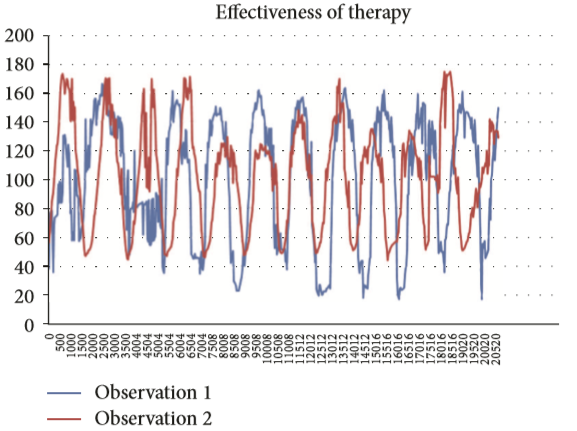
\includegraphics[width=110mm]{rahman_viz.png}
\caption{Visualization used in \cite{rahman} depicting the degree of forearm movement overtime}
\label{rahman_viz}
\end{figure}

\begin{figure}
\centering
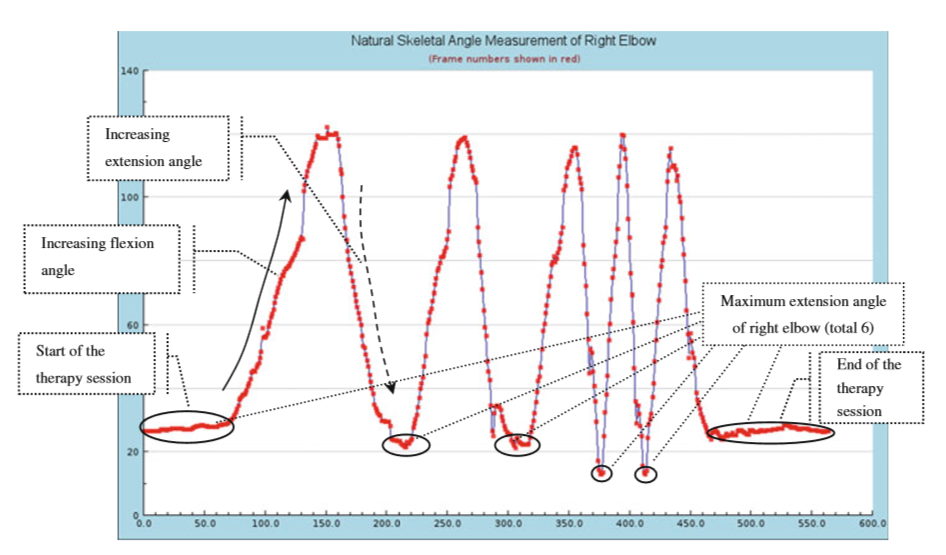
\includegraphics[width=150mm]{rahman2_elbowangle.png}
\caption{Visualization used in \cite{rahman2} depicting the speed of movement (m/s) of forearm overtime}
\label{rahman2}
\end{figure}

In \cite{green}, a virtual reality rehabilitation system for children with hemiplegia was developed using TUI\footnote{\url{https://en.wikipedia.org/wiki/Tangible_user_interface}}. The game itself is displayed on LCD and the player interact with the game by placing the TUI on top of moving targets shown on the LCD. In this system, performances are measured by speed, accuracy and trajectory(mean movement efficiency). However, unlike \cite{rahman}, this system doesn't provide an interface in which therapist can analyse the gameplay.

Similar to Hammer and Planks, \cite{rahman2} introduced a framework which uses Kinect attached to Second Life\footnote{\url{http://secondlife.com/}} serious game environment. The mission of the game is to follow a set of movement that have been configured beforehand by the therapist. During the game, the movement of each body joint  is recorded and saved in Session Recorder. Afterwards, a Kinematic Analytic component will process this data and visualize the quality of improvement metrics of each body joint movement. Each metric is visualized with a dotted line chart over time as shown in Figure \ref{rahman2}. Even though it's possible to  see which line curve indicate an elbow flexion or extension, the therapist needs to count the number of the curve manually. This is not very efficient when the session is longer and there are more curve to count.

\section{Visualization of Time Series Data}

Since one of the requirement of the interface is to have the information of movement evolution over time, it is interesting to review how a time series data is usually visualized. Tominski and Aigner discuss at length about the techniques of time series data visualization in their book\cite{aigner}. The visual survey of this book can be found on their website\footnote{\url{http://survey.timeviz.net}}. This section reviews some of these interesting techniques.

Considering that the recorded gameplay data contains spatial information (location of an event happened on the screen), we reviewed techniques which concern visualizing spatio-temporal data. \textbf{Flow Map} depicts movements of object over time. Object movements are usually represented by directed trajectories over spatial space(i.e: map) with different color, width, angle of trajectories represent additional information. In order to overcome overlapping trajectories for huge amount of data, usually aggregation techniques (clustering, self organizing map, etc.) are introduced to group similar data point. Figure \ref{flow_map} shows an example of flow map depicting photographers movement between cities in Germany \cite{adrienko}. In this case, the aggregation considers three parameters: initial location, destination location, and time period in which the movement happened. Trajectories width indicate the number of photographers who move between the cities. Another visualization technique worth to mention is \textbf{Spatio-Temporal Event Visualization} which uses the space-time cube concept. In this concept, the x and y axis usually represent two spatial dimensions while the third axis represent temporal dimension. The events are then represented as graphical objects which are mapped to the space-time cube location. Different events attribute can be represented in different size, colors, shape, or texture. Figure \ref{spatio_temporal} shows space-time cube which depict convective clouds \cite{turdukulov}, human health \cite{tominski} and earthquake events \cite{gatalsky} from left to right. As we can see, the  spatial dimension of the left chart is area in pixel while the middle and right chart is a map. The events on the chart are represented with sphere objects with different color and different sizes. Even though space-time cube can portrays the spatio-temporal data, it has some downside. When there are too many events, occlusion is inevitable. It should be coupled with an appropriate interaction technique to allow users see the data from different perspective.

\begin{figure}
\centering
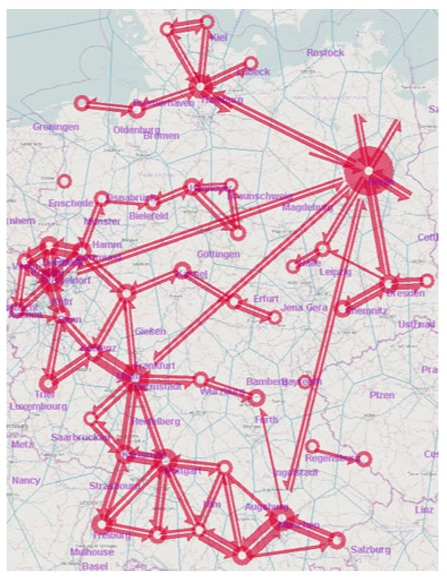
\includegraphics[width=90mm]{aigner_flowmap.jpg}
\caption{Flow Map}
\label{flow_map}
\end{figure}

\begin{figure}
\centering
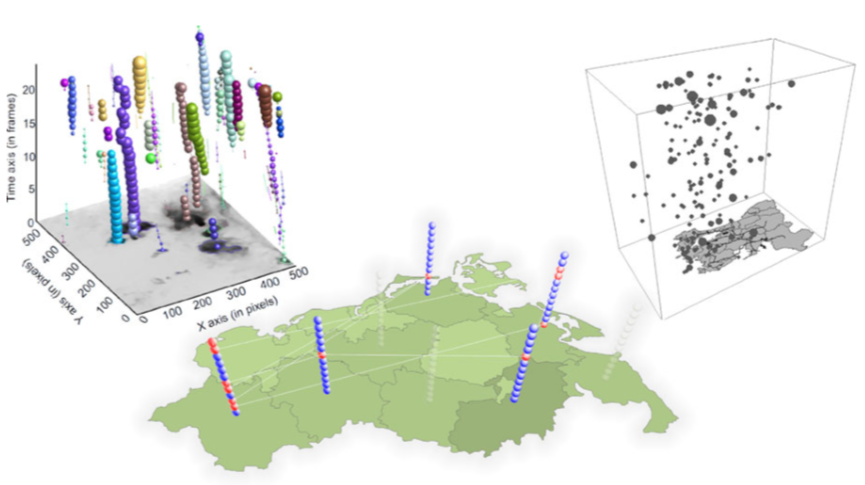
\includegraphics[width=150mm]{aigner_spatiotemporaleventviz.png}
\caption{Spatio-Temporal Event Visualization}
\label{spatio_temporal}
\end{figure}

One example of time-series visualization technique which doesn't concern spatial data is Theme River. First introduced in \cite{havre}, Theme River is used to visualize thematic changes over time of document collection. Each theme is represented as different colors which flows from left to right with different width over different time point. The width depicts theme strength over temporal axis. The purpose of this technique was to easily understand the evolution of theme strength over time. Figure \ref{themeriver} shows an example of Theme River representation of 1990 Associated Press newswire data. It can be seen on the chart that the theme baghdad, saddam, iraq, and kuwait are gaining strength  around the time Iraq invaded Kuwait on August 2, 1990. By following the flow of a certain color (theme) we can easily see the changes in theme strength and associate it with the events that affects the changes. Theme River should be supported with interaction techniques which allow user to rearrange river positioning over horizontal axis. 

Consequently, the Theme River technique is chosen due to its ability to show evolution of a certain data variable over time. Further details on the implementation can be found on Chapter 4.

\begin{figure}
\centering
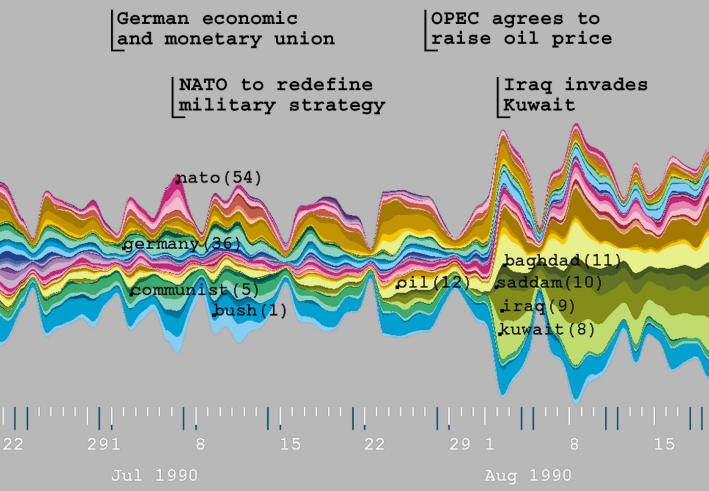
\includegraphics[width=150mm]{havre_themeriver.png}
\caption{Theme River}
\label{themeriver}
\end{figure}


\section{Visualization of Movement Data}

Movement data usually represents an object which moves over a certain space \cite{adrienko_book}: data of moving car, birds migration, etc. It's usually recorded as series of location (latitude/longitude, x/y coordinates, etc.) and time. On the other hand, body movement data are recorded as vector representation of human pose \cite{bernard2013} over time. On this section, we first review visualization for movement data in general and then discuss visualization for body movement focusing on visualization for skeleton animation\footnote{\url{https://en.wikipedia.org/wiki/Skeletal_animation)}} data.

There have been numerous method and application developed to analyse movement data. \cite{adrienko} gives an overview on these methods and applications. Movement data for discrete entities are usually represented as linear symbol over a map or space time cube. However, this technique has problem with occlusions for huge amount of data. Therefore, it's usually accompanied with other graph such as time graph. Other solution to this problem is to use clustering on the trajectories. Apart from minimizing the number of trajectories presented on the view at the same time, clustering also help user to find interesting pattern of the movement. Figure \ref{car_trajectory} \cite{adrienko_book} gives an example of trajectories of a single car from gps data over several days. The trajectories are divided by stop duration at least 3 hours and clustered by route similarity represented in different colors. Therefore, it is possible to know which route are often or less taken by car owner.

\begin{figure}
\centering
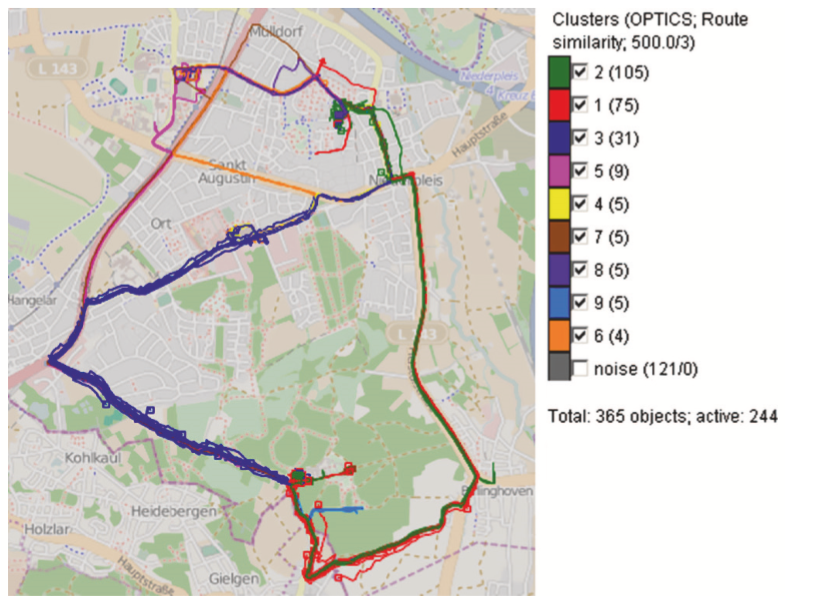
\includegraphics[width=150mm]{adrienko_clustered.png}
\caption{Car Trajectories clustered by route similarity}
\label{car_trajectory}
\end{figure}

Patterns can also be found by introducing aggregation and generalisation technique on spatial or temporal properties of the movement. For example, the movement data can be aggregated spatially into a discrete grid and for each grid, the number of movement (total or average) happened within the grid can be represented with color or objects in different size. Figure \ref{car_milan} \cite{adrienko_book} shows the presence of cars in Milan in certain geographical area (generated with Voronoi tessellation \cite{okabe}) during certain time period. The number of cars in the area is represented with a circle in different size which indicate intensity of traffic. As we can see, there are more traffic between 05-06h (left) compared to 22-23h (right). This is understandable since most people leave work around 5  to 6 pm and are already home at 22-23 pm.

\begin{figure}
\centering
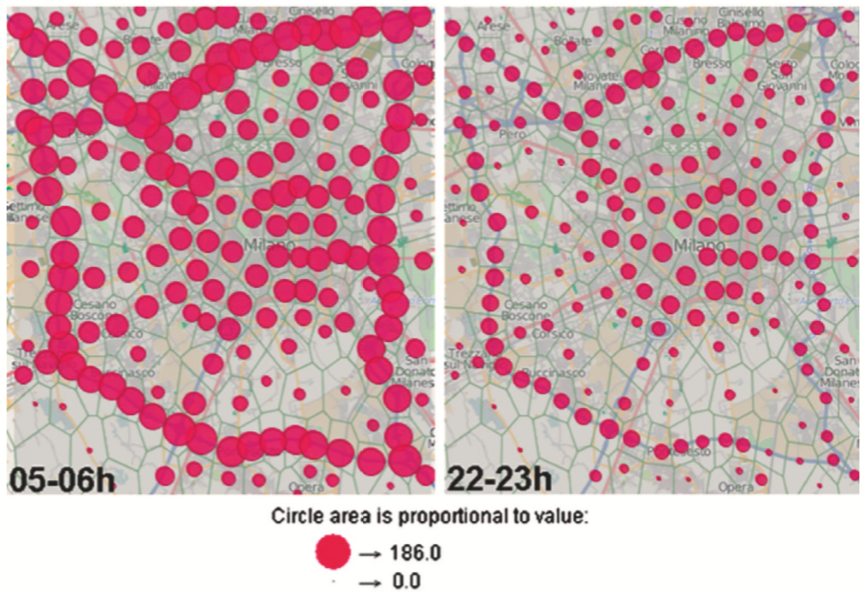
\includegraphics[width=150mm]{adrienko_milan.png}
\caption{Presence of cars in Milan in different time period}
\label{car_milan}
\end{figure}

Recognizing and understanding human movement has many benefits in different application domain: arts\cite{heryadi,raptis}, sports\cite{bernard2013}, healthcare\cite{patsadu}, etc. There are numerous research has been done concerning human movement analysis as discussed in  \cite{gavrila} which surveyed different methodologies and approaches. Most of the methodologies discussed focus on identifying a certain type of movement. On the other hand, to our knowledge, there hasn't been many research which focus on human body movement visualization in which user can explore and analyse a certain data set. 

\cite{chmelik} proposes a system to track and visualize body movement on a virtual environment in real time. In this system, body parts  which desired to be tracked are attached to an optical system with twelve infrared cameras. Once user move the tracked body parts, a "motion trail" will be shown in the virtual environment in which then user can manipulate its representation by changing the color, shape, smoothness, etc. These interaction also conducted directly in the virtual environment. Figure \ref{motion_trail} \cite{chmelik} shows the motion trail produced in the virtual environment while a user move the tracking device in his hand. On the right is the interface where user can interact with the visualization.

Another approach to visualize body movement is by using color belt \cite{yuko}. In this approach, movement data collected from motion capture system with 11 sensors attached in body joints (Figure \ref{color_belt} left) are grouped into 4 limbs movement: Right Arm, Left Arm, Right Leg, Left Leg. Each of the limb representation is arranged in vertical axis sequentially forming a belt. The horizontal axis represents time (from left to right) and the sections represent sets of movement. Limb motions are shown as gradation of red-green colors in this belt by extracting the position and angle of associated body joints data (Figure \ref{color_belt} middle). Positive angle is represented with red color, while negative angle is represented with green color. Figure \ref{color_belt} (right) shows a color belt and how it is related to the body movement done by a gymnast. The color belt shows the first to fourth movement set. As can be seen in the picture, the gymnast move her leg on the second exercise and the second section on the color belt depicts the movement for right leg and left leg.

\begin{figure}
\centering
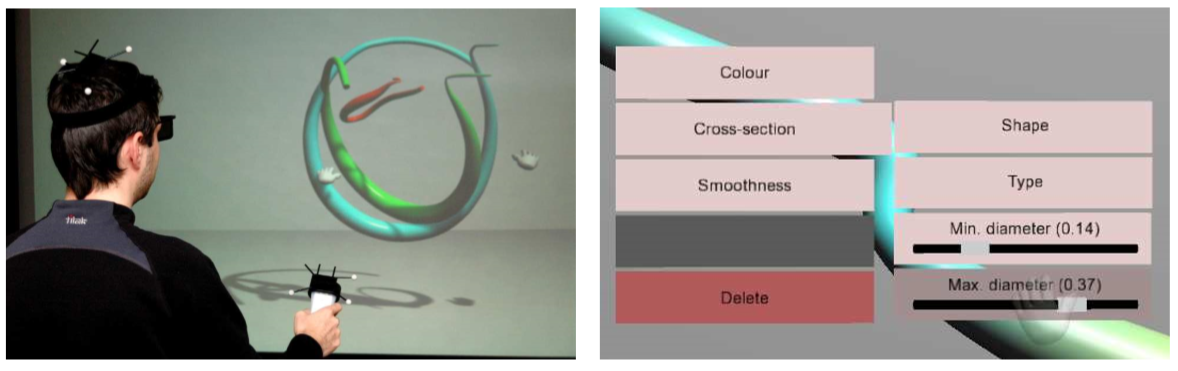
\includegraphics[width=150mm]{chmelik_trail.png}
\caption{Motion Trail}
\label{motion_trail}
\end{figure}

\begin{figure}
\centering
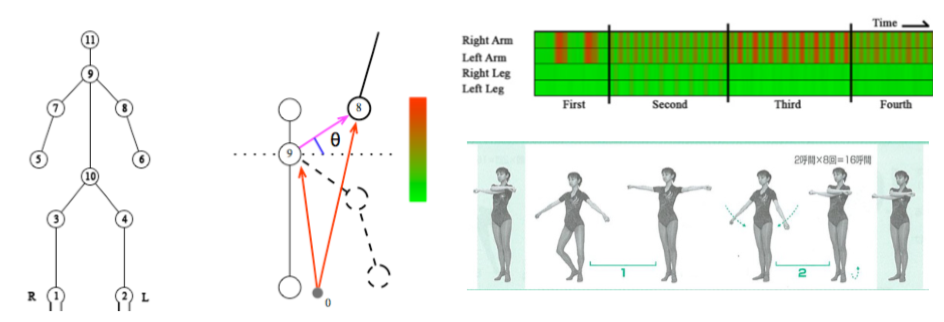
\includegraphics[width=150mm]{yuko_belt.png}
\caption{Color Belt depicting gymnast body movement}
\label{color_belt}
\end{figure}

MotionExplorer\cite{bernard2013} introduced human motion exploratory search using hierarchical aggregation. This approach are directed towards the need to explore huge quantity of motion data and be able to identify interesting sequence of movements. Implemented on database which contains various motions in multiple repetitions, first each human pose data is clustered using k-means algorithm. A pose cluster comprises of a large numbers of similar human pose and is represented as a circular glyph with human stick-figure pose as the centroid and set of pose in the cluster as deviating, transparent figures. The cycle around cluster glyph are colored based on color legend and shows similarity among clusters. MotionExplorer provides 4 views (Figure \ref{motion_explorer}): (i) \textit{Pose hierarchy explorer} (top left) allows user to explore all available pose cluster in the data sets hierarchically. The pose cluster hierarchy is shown as a dendogram and calculated with a divisive clustering algorithm. The aggregation level is adjustable. (ii) \textit{Motion explorer} (top right) shows sequences between pose clusters at current aggregation level. Human poses are represented as nodes while edges represent motion sequences. Two nodes are connected if there is at least one motion sequence which connects both pose clusters. (iii) \textit{Motion search} interface (bottom right) allows user to input query for a specific motion sequence by inputting start pose and end pose. An interactive search result is provided where user can explore each style variations. The interface is divided into 4 parts: start pose field, search result field, end pose field and pose bundle animation. A user can make search query by choosing/dragging a pose cluster to the start and end pose field. The resulting motion sequences are then shown in the search result field on the granularity of a single human pose. (iv) \textit{Pose color mapping} (box on bottom left) is a color legend related to each pose cluster. The color grid is built using SOM algorithm trained with all feature vectors in a vector quantization scheme. By clicking one of the clusters in the color legend, the aggregation level will be adjusted to the granularity level of the selected pose cluster. Each visualization window is linked. When user changes the aggregation level in the pose hierarchy explorer, the motion explorer is automatically adjusted to the new aggregation level. When user clicks on one of the clusters in the color legend, the system automatically adjust the aggregation level to the same granularity of the selected cluster. If a cluster in one of the view is selected, then the same cluster pose is also highlighted in every view. 

\begin{figure}
\centering
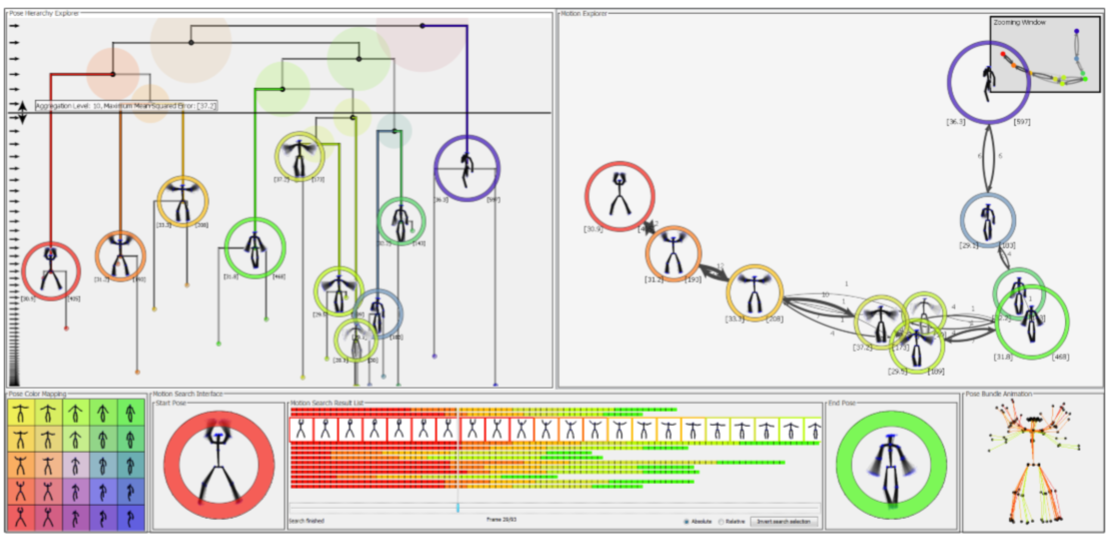
\includegraphics[width=150mm]{bernard_motionexplorer.png}
\caption{MotionExplorer interface}
\label{motion_explorer}
\end{figure}

\section{D3.js as Data Visualization Tool}

The popularity of data visualization has been supported with the development of a lot of data visualization tool. To support the development of the interface in this thesis, a survey were conducted focusing on tools which allows creation of different visualization technique without restriction of a ready made template or certain chart type. 

One of the tools surveyed is D3\cite{bostock}. \textbf{D3} or Data-Driven Documents is a javascript library which allows user to create desired visualization either the standard one (bar, line, scatter plot, etc.) or the customized one (limited only by one's creativity) in 2D. Built by incorporating HTML5, CSS, and SVG standards, D3 enables user to load data in various format(.json,.csv,.txt, etc.)\footnote{\url{https://github.com/mbostock/d3/wiki/API-Reference}} and present it as a chart. The various functionality offered by D3 and its detailed API documentation has encourage a lot of people to explore it. This resulted in numerous amount of D3 demo online which can be a good reference source for new user\footnote{\url{http://techslides.com/over-2000-d3-js-examples-and-demos}}. Thus, starting using D3 is quite easy with so many example online supported with big community. On top of that, D3 provides different ways to manipulate and interact with the data which enables development of interactive and intuitive visualization. Figure \ref{d3_example} shows some of the visualizations built in D3\footnote{\url{http://d3js.org}}. Considering the visualization requirement identified in the previous chapter as well as the features offered by D3, consequently D3 is chosen as the tool for interface development in this thesis.

\begin{figure}
\centering
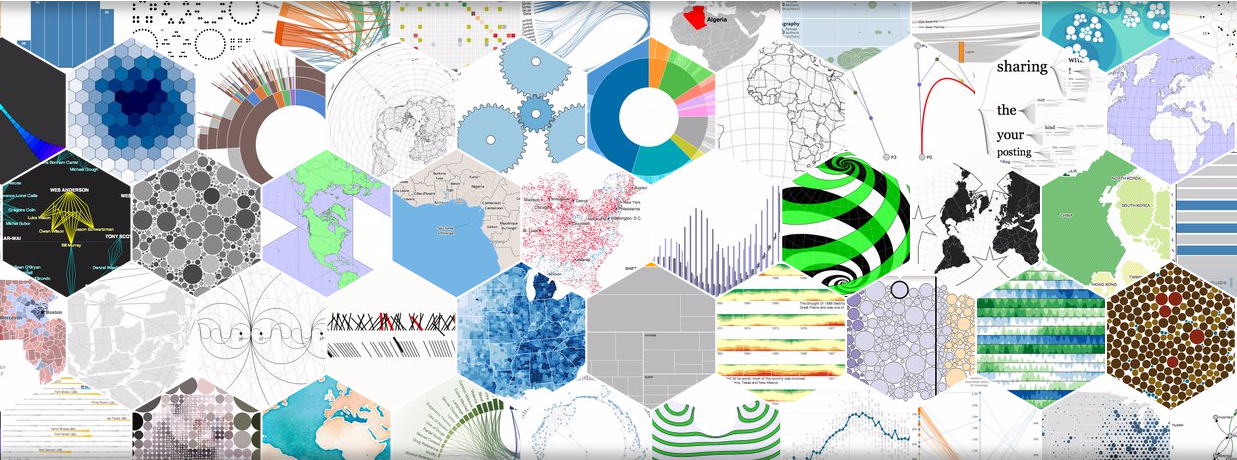
\includegraphics[width=100mm]{d3js.png}
\caption{Some of visualizations developed with D3.js}
\label{d3_example}
\end{figure}










